\begin{figure*}[ht]
\centering

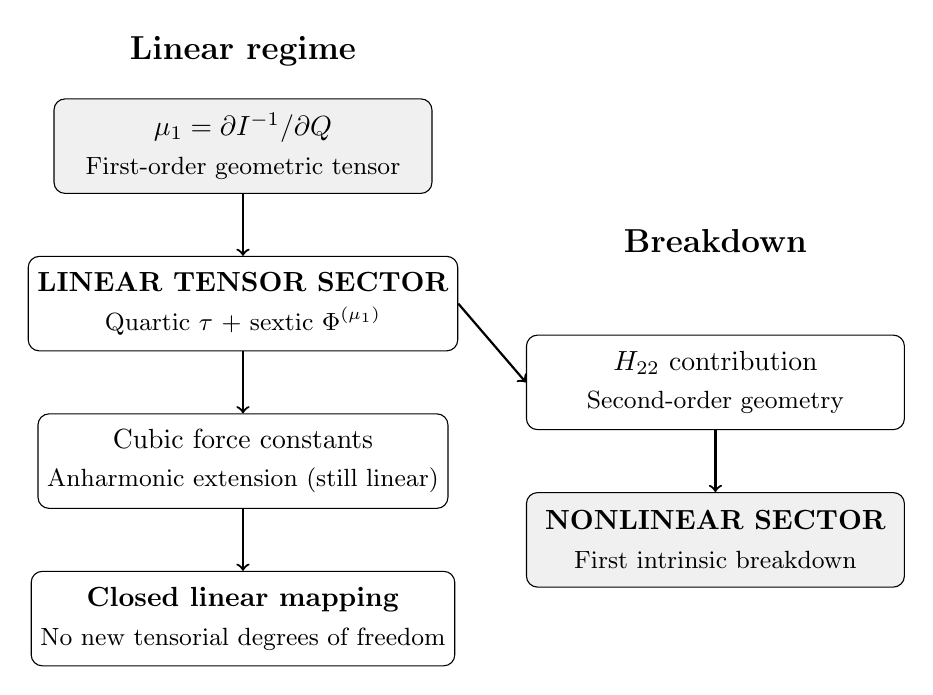
\begin{tikzpicture}[
box/.style={
rectangle,draw,rounded corners,
align=center,
minimum width=4.8cm,
minimum height=1.2cm
},
core/.style={
rectangle,draw,rounded corners,
align=center,
minimum width=4.8cm,
minimum height=1.2cm,
fill=gray!12
},
arrow/.style={->, thick}
]

% =======================
% LEFT COLUMN (LINEAR SECTOR)
% =======================

\node[core] (mu1) at (0,0)
{$\mu_1 = \partial I^{-1} / \partial Q$ \\[2pt]
\small First-order geometric tensor};

\node[box] (linear) at (0,-2)
{\textbf{LINEAR TENSOR SECTOR} \\[2pt]
\small Quartic $\tau$ + sextic $\Phi^{(\mu_1)}$};

\node[box] (cubic) at (0,-4)
{Cubic force constants \\[2pt]
\small Anharmonic extension (still linear)};

\node[box] (closed) at (0,-6)
{\textbf{Closed linear mapping} \\[2pt]
\small No new tensorial degrees of freedom};

% =======================
% RIGHT COLUMN (BREAKDOWN)
% =======================

\node[box] (h22) at (6,-3)
{$H_{22}$ contribution \\[2pt]
\small Second-order geometry};

\node[core] (nonlinear) at (6,-5)
{\textbf{NONLINEAR SECTOR} \\[2pt]
\small First intrinsic breakdown};

% =======================
% ARROWS
% =======================

\draw[arrow] (mu1) -- (linear);
\draw[arrow] (linear) -- (cubic);
\draw[arrow] (cubic) -- (closed);

\draw[arrow] (linear.east) -- (h22.west);
\draw[arrow] (h22) -- (nonlinear);

% =======================
% LABELS
% =======================

\node at (0,1.2) {\large \textbf{Linear regime}};
\node at (6,-1.2) {\large \textbf{Breakdown}};

\end{tikzpicture}

\caption{
Conceptual organization of centrifugal-distortion contributions within the tensor framework. The first derivatives of the inverse inertia tensor ($\mu_1$) generate a linear tensor space that fully determines both standard quartic and sextic centrifugal distortion constants. Anharmonic contributions arising from cubic force constants extend the physical content while remaining within the same linear mapping, so that the linear sector remains closed. The first intrinsic breakdown arises from the $H_{22}$ contribution, which introduces a second-level geometric tensor and defines the onset of a nonlinear tensor sector.
}

\label{fig:tensor_hierarchy}

\end{figure*}
